\part*{Task 2: Identify User, Software, and System Requirements}
\addcontentsline{toc}{part}{Task 2: - Identify User, Software, and System Requirements}

The identification of user, software, and system requirements were scraped and
    analyzed from the Google Play Store, both from the app's description and its
    reviews.

\section*{Analyzing GrandPad's Google Play Reviews}
\addcontentsline{toc}{section}{Analyzing GrandPad's Google Play Reviews}

The following explanation of the analysis of GrandPad's reviews is a summary of
    the Jupyter Notebook in Appendix \ref{sec:reviews_processing_notebook}.

Using the
    \href{https://pypi.org/project/google-play-scraper/}{google-play-scraper}
    Python library, reviews were scraped from the Google Play Store.
Initially, 1,823 reviews were scraped, many of which were under 10 words.
This is shown in the histogram below.
\begin{figure}[H]
    \centering
    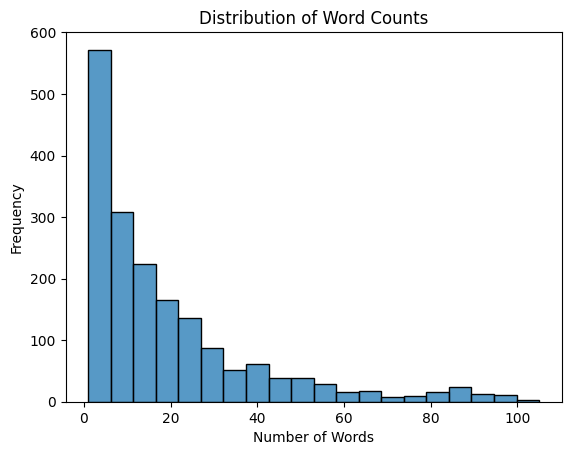
\includegraphics[width=0.75\textwidth]{images/word_length_distribution.png}
\end{figure}
To reduce the amount of data to analyze, all reviews under 10 words were
    removed.
The reviews were then split by their rating (5 stars: positive, 2-4 stars:
    mixed, 1 star: negative) and run through a
    \href
        {https://scikit-learn.org/dev/modules/generated/sklearn.decomposition.LatentDirichletAllocation.html}
        {Latent Dirichlet Allocation (LDA) algorithm from Scikit Learn}
    to identify important topics from each category of the reviews.

\subsection*{User Requirements from Negative Reviews}
\addcontentsline{toc}{subsection}{User Requirements from Negative Reviews}

The analysis of negative reviews led to some recurring topics, which included
    lack of professional support,
    intrusive app behavior,
    lack of personalization functionality,
    poor quality of video and voice calls,
    and frustrating notification experience.

\begin{description}
    \item[\textbf{USER-\showmycounter}]
        As a member of a GrandPad family network, I need to have access to
            support staff during work hours to help configure the network.
    \item[\textbf{USER-\showmycounter}]
        As a senior user of GrandPad, I need to have access to support staff
            during work hours to help troubleshoot problems with the GrandPad
            tablet.
    \item[\textbf{USER-\showmycounter}]
        As a user of the GrandPad app, I don't want the app to override
            Do Not Disturb mode on my phone.
    \item[\textbf{USER-\showmycounter}]
        As an administrator of a GrandPad network, I want to be able to
            customize the elderly user's GrandPad tablet to suit their
            proficiency and comfort levels with technology.
    \item[\textbf{USER-\showmycounter}]
        As an elderly user of the GrandPad tablet who is moderately comfortable
            with technology, I want to be able to customize the my GrandPad
            tablet to add or remove features.
    \item[\textbf{USER-\showmycounter}]
        As a member of a GrandPad family network, I want to video call with high
            enough quality to see and hear my loved ones.
    \item[\textbf{USER-\showmycounter}]
        As a member of a GrandPad family network, I want to voice call with high
            enough quality to hear my loved ones.
    \item[\textbf{USER-\showmycounter}]
        As a user of the GrandPad app, I want to be able to receive
            notifications when a member of the network posts, comments, or
            reacts to a post, or calls me.
    \item[\textbf{USER-\showmycounter}]
        As a user of the GrandPad app, I want to be able to clear all
            notifications at once, without having to individually clear each
            one.
\end{description}

\subsection*{User Requirements from Mixed Reviews}
\addcontentsline{toc}{subsection}{User Requirements from Mixed Reviews}

When analyzing the mixed reviews, some recurring topics were
    connecting multiple GrandPad tablets to a single network,
    being part of multiple networks,
    editing posts and comments,
    vague error messages,
    posting multiple files at once,
    and sending message to or calling specific people in a network.

\begin{description}
    \item[\textbf{USER-\showmycounter}]
        As an administrator of a GrandPad family network, I need to be able to
            add multiple users with GrandPad tablets to a single member, to
            accommodate multiple elderly family members.
    \item[\textbf{USER-\showmycounter}]
        As a user of the GrandPad app, I want to be able to easily join and
            switch between multiple GrandPad family networks to be part of
            multiple groups of people.
\end{description}

\subsection*{User Requirements from Positive Reviews}
\addcontentsline{toc}{subsection}{User Requirements from Positive Reviews}

When analyzing positive reviews, prominent topics that were found include
    test.

\begin{description}
    \item[\textbf{USER-\showmycounter}]
        test
\end{description}
